\documentclass[border=10pt]{standalone}

\usepackage{tikz}
\usepackage{tikzsymbols}
\usetikzlibrary{calc,patterns,shapes.geometric}

\def\centerarc[#1](#2)(#3:#4:#5){\draw[#1] ($(#2)+({#5*cos(#3)},{#5*sin(#3)})$) arc (#3:#4:#5);}

\begin{document}
	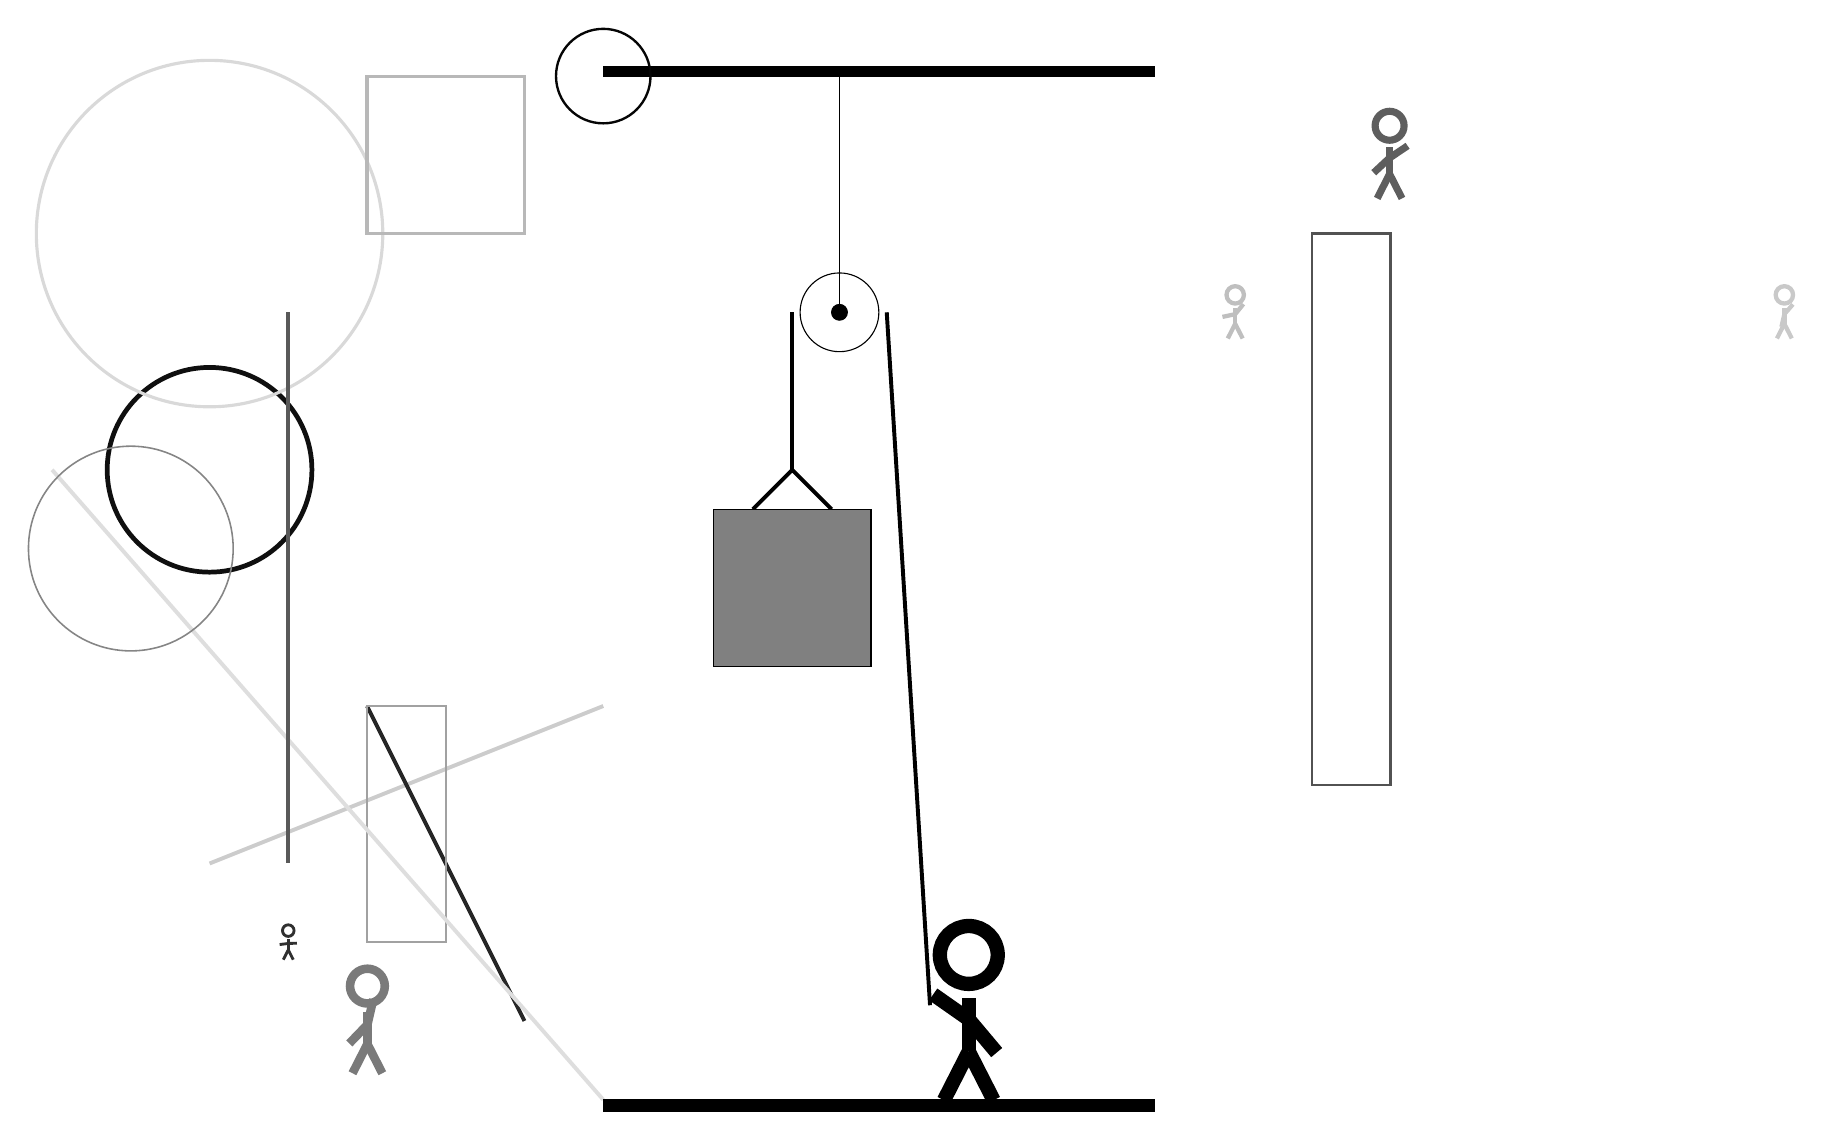
\begin{tikzpicture}
		%%%%% START %%%%%
		
		\draw[fill=black] (-2, 10) rectangle (5, 10.125);
		
		\draw (1, 7) circle (0.5);
		\draw[fill=black] (1, 7) circle (0.1);
		\draw (1, 10) -- (1, 7);
		
		\draw[line width=0.5mm] (-0.1, 4.5) -- (0.4, 5.0) -- (0.9, 4.5);
		\draw[fill=black!50] (-0.6, 4.5) rectangle (1.4, 2.5);
		
		\draw[line width=0.5mm] (0.4, 7) -- (0.4, 5.0);
		\centerarc[line width=0.5mm](1, 7)(0:180:0.6);
		\draw[line width=0.5mm](1.6, 7) -- (2.15, -1.8);
		
		\draw[line width=0.5mm, color=black!20](-2, 2) -- (-7, 0);
		
		\node[line width=0.5mm, color=black!63] at (8, 9) {\Strichmaxerl[5][43][34]};
		\draw[line width=0.5mm, color=black!85](-5, 2) -- (-3, -2);
		\node[line width=0.6mm, color=black!52] at (-5, -2) {\Strichmaxerl[6][46][77]};
		\draw[line width=0.2mm, color=black!37] (-4, 2) rectangle (-5, -1);
		\draw [line width=0.6mm, color=black!94](-7, 5) circle (1.3);
		\draw[line width=0.3mm, color=black!68] (7, 8) rectangle (8, 1);
		\node[line width=0.5mm, color=black!25] at (6, 7) {\Strichmaxerl[3][12][51]};
		\node[line width=0.6mm, color=black!81] at (-6, -1) {\Strichmaxerl[2][7][2]};
		\draw [line width=0.4mm, color=black!15](-7, 8) circle (2.2);
		\draw[line width=0.5mm, color=black!13](-2, -3) -- (-9, 5);
		
		\draw[line width=0.5mm, color=black!65](-6, 7) -- (-6, 0);
		\draw [line width=0.2mm, color=black!48](-8, 4) circle (1.3);
		\draw[line width=0.4mm, color=black!28] (-3, 8) rectangle (-5, 10);
		\node[line width=0.4mm, color=black!21] at (13, 7) {\Strichmaxerl[3][77][49]};
		\draw [line width=0.3mm, color=black!98](-2, 10) circle (0.6);
		
		
		\node at (2.6, -1.9) {\Strichmaxerl[10][-35][-50]};
		
		\draw[fill=black] (-2, -3) rectangle (5, -3.15);
		
		%%%%% END %%%%%
	\end{tikzpicture}
\end{document}